\documentclass[conference]{IEEEtran}
\usepackage{ifpdf}
\usepackage{booktabs}
\usepackage{cite}
\usepackage[cmex10]{amsmath}
\usepackage{amsfonts}
\usepackage{url}
\usepackage{color}
\usepackage[utf8]{inputenc}
\usepackage{algpseudocode}
\usepackage{algorithm}
\usepackage{booktabs}
\usepackage{tabularx}
\usepackage{multicol}
\usepackage{bm}
\usepackage{multirow}
\usepackage{array}
\usepackage{epstopdf}
\ifCLASSINFOpdf
   \usepackage[pdftex]{graphicx}
  % declare the path(s) where your graphic files are
   \graphicspath{{figures/png/}}
  % and their extensions so you won't have to specify these with
  % every instance of \includegraphics
  \DeclareGraphicsExtensions{.png}
\else
  % or other class option (dvipsone, dvipdf, if not using dvips). graphicx
  % will default to the driver specified in the system graphics.cfg if no
  % driver is specified.
  \usepackage[dvips]{graphicx}
  % declare the path(s) where your graphic files are
  \graphicspath{{figures/eps/}}
  % and their extensions so you won't have to specify these with
  % every instance of \includegraphics
  \DeclareGraphicsExtensions{.eps}
\fi
\usepackage{epsfig}
\newcolumntype{M}{>{$\vcenter\bgroup\hbox\bgroup}c<{\egroup\egroup$}}
\newcommand{\etal}{\textit{et al.}}
\begin{document}
%
% paper title
% Titles are generally capitalized except for words such as a, an, and, as,
% at, but, by, for, in, nor, of, on, or, the, to and up, which are usually
% not capitalized unless they are the first or last word of the title.
% Linebreaks \\ can be used within to get better formatting as desired.
% Do not put math or special symbols in the title.
\title{A Sparse regularization approach for ultrafast ultrasound imaging}

\author{\IEEEauthorblockN{Rafael E. Carrillo\IEEEauthorrefmark{1}\IEEEauthorrefmark{4},
Adrien Besson\IEEEauthorrefmark{1}\IEEEauthorrefmark{3},
Miaomiao Zhang\IEEEauthorrefmark{2}, 
Denis Friboulet\IEEEauthorrefmark{2},
Yves Wiaux\IEEEauthorrefmark{3},}
Jean-Philippe Thiran\IEEEauthorrefmark{1}\IEEEauthorrefmark{4} and
Olivier Bernard\IEEEauthorrefmark{2}
\IEEEauthorblockA{\IEEEauthorrefmark{1}Signal Processing Laboratory (LTS5),
Ecole Polytechnique F\'{e}d\'{e}rale de Lausanne,
Lausanne, Switzerland\\}
\IEEEauthorblockA{\IEEEauthorrefmark{2}CREATIS, CNRS UMR5220, University of Lyon, INSA-Lyon, University of Lyon1, Villeurbanne, France}
\IEEEauthorblockA{\IEEEauthorrefmark{3}Institute of Sensors, Signals and Systems, Heriot-Watt University, Edinburgh, UK\\}
\IEEEauthorblockA{\IEEEauthorrefmark{4}Department of Radiology, University Hospital Center (CHUV) and University of Lausanne (UNIL), Lausanne, Switzerland}}
\maketitle

\begin{abstract}
Ultrafast imaging based on plane-wave (PW) insonification is an active area of research due to its capability of reaching high frame rates. Several approaches have been proposed either based on either of Fourier-domain reconstruction or on delay-and-sum (DAS) reconstruction. Using a single PW, these techniques achieve low quality, in terms of resolution and contrast, compared to the classic DAS method with focused beams. To overcome this drawback, compounding of several steered PWs is needed, which currently decreases the high frame rate limit that could be reached by such techniques. Based on a compressed sensing (CS) framework, we propose a new method that allows the reconstruction of high quality ultrasound (US) images from only 1 PW at the expense of augmenting the computational complexity at the reconstruction.
\end{abstract}

\begin{IEEEkeywords}
Plane wave, Fourier imaging, Ultrafast imaging, Sparsity, Compressed sensing
\end{IEEEkeywords}

\IEEEpeerreviewmaketitle



\section{Introduction}
\par Ultrafast ultrasound (US) imaging faces an increasing interest in the ultrasound community due to its capability to perform very high frame rate imaging with image quality comparable to the one obtained with conventional techniques. The principle is to use one or several steered plane waves to insonify the medium. Thus, the only limitation in the frame rate is the time the sound wave spends to insonify the medium. The existing ultrafast methods can be classified in two categories: spatial-based approaches where the desired image is obtained from a delay-and-sum (DAS) beamforming in the space-domain~\cite{Montaldo_UFFC_2014,Papadacci_uffc_2014} and Fourier-based techniques where the received raw-data are used to reconstruct the Fourier spectrum of the image of interest~\cite{Lu_UFFC_97,garcia_uffc_2013,Bernard_IUS_2014}. In this study, we focus on the second group of methods. In these techniques, the following generic scheme is used. One or several plane waves are first emitted. Backscattered echoes are then measured. 2D-Fourier transform is applied on the received image and non-evanescence acoustic wave properties are then applied. Finally, an adjoint Non-Uniform Fourier Transform (frequency remapping and inverse Fourier Transform) is applied to come back to the desired image space.

\par One important shared property of the above mentioned methods is that they all need a frequency remapping to project the echo k-space onto the desired image k-space. This frequency remapping leads to inaccuracies due to model approximation as well as interpolation errors which induce degradation of the final image. Compressed sensing (CS) is a mathematical framework to recover signals from incomplete information~\cite{Donoho_TIT_2006,candes06,fornasier11} that has been successfully applied to medical US imaging (see \cite{Friboulet_IUS_2010} and references therein). In this paper, we propose a new imaging method based on a CS framework that allows recovering high quality images. The proposed method reformulates the Fourier beamforming process as a linear inverse problem and exploits sparsity of US images in a redundant dictionary as a regularization. To recover the US image an $\ell_1$ minimization problem is posed and an efficient algorithm is used to solve it.

\par The paper is organized as follows. Section \ref{sec:Back} briefly reviews the Ultrasound Fourier Slice Beamforming (UFSB) method and the mathematical principles of the CS framework. Section \ref{sec:S-UFSB} presents the proposed sparse regularization approach for ultrafast US imaging. Experiments comparing the quality of the proposed method to state of the art methods in plane-wave (PW) imaging are presented in section \ref{sec:Exp}. Finally, concluding remarks are given in section \ref{sec:Conc}. 

\section{Background}
\label{sec:Back}
\subsection{Ultrasound Fourier slice beamforming}
\label{ssec:UFSB}
The key idea of the UFSB method is to use steered plane waves, both in emission and in reception, and to exploit Fourier slice theory to recover the desired US image~\cite{Bernard_IUS_2014}. Suppose we have a linear array composed by $N_t$ transducers. Define $s(t)=\sum_{i=1}^{N_t}s_i(t)$, where $s_i(t)$ denotes the received echo by the $i$-th transducer. Bernard \etal \: show in \cite{Bernard_IUS_2014} that the temporal Fourier transform of $s(t)$ corresponds to the 2D spatial Fourier transform of the image restricted to a radial line in a given direction.  

More precisely, suppose the emitting plane wave has normal incidence, i.e. $n_e = [0, 1]^T$, and that the receiving plane wave is steered with angle $\xi_r$, i.e. $n_r = [sin \xi_r, cos \xi_r]^T$. Then the temporal Fourier transform of $s(t)$ (received with angle $\xi_r$) corresponds to a radial line in the k-space representation (spectrum) of the desired image. The line is characterized by: 
\begin{align}
\left\lbrace
\begin{array}{l l}
k_x &= k \sin ( \xi_r )\\
k_z &= k \left( 1+ \cos ( \xi_r ) \right) 
\end{array}
\right.
\end{align}
where $k=2\pi f/c$ is the wave number in the direction $n_{er}=n_e+n_r$. The direction of the radial line in k-space is given by $\theta_r= \frac{\xi_r}{2}$. Thus, it is possible to recover the desired image by populating the image spectrum with various $\xi_r$ at reception for the same emitting angle and by applying an inverse Fourier transform to come back from the non-uniformly sampled k-space $\left( k_x, k_z \right)$ to the desired image space.

\subsection{Compressed sensing framework}
\label{ssec:CS}
The now famous theory of compressed sensing (CS) introduces a signal acquisition framework that goes beyond the traditional Nyquist sampling paradigm\cite{Donoho_TIT_2006,candes06,fornasier11}. Let $\bm{x} \in \mathbb{C}^{N}$ be the signal under scrutiny. The fundamental premise in CS is that certain classes of signals, such as natural images, have a concise representation in terms of a sparsity dictionary $\mathsf{\Psi}$,  such that $\bm{x} = \mathsf{\Psi}\bm{\alpha}$, where most of the coefficients $\bm{\alpha}$ are zero, or small, and only few are significant. CS demonstrates that such sparse or compressible signals can be acquired using a small number of linear measurements and then recovered by solving a non-linear optimization problem~\cite{candes06,Donoho_TIT_2006,fornasier11}. 

Formally, the signal $\bm{x}$ is measured through the linear model $\bm{y}=\mathsf{\Phi}\bm{x}+\bm{n}$, where $\bm{y}\in\mathbb{C}^{M}$ denotes the measurement vector, $\mathsf{\Phi}\in\mathbb{C}^{M\times N}$, $M<N$, is the sensing matrix and $\bm{n}\in\mathbb{C}^{M}$ represents the observation noise (or model inaccuracies). Recovering $\bm{x}$ from $\bm{y}$ poses an ill-posed linear inverse problem where the sparse prior on the signal regularizes the solution. CS shows that the following convex problem can recover $\bm{x}$ under certain conditions of the matrix $\mathsf{\Phi}$~\cite{candes11}:
%
\begin{equation}\label{cs6}
\min_{\bar{\bm{x}}\in\mathbb{C}^{N}}\|\mathsf{\Psi}^{\dagger}\bar{\bm{x}}\|_{1}
\textnormal{ subject to }\| \bm{y}-\mathsf{\Phi}\bar{\bm{x}}\|_{2}\leq\epsilon,
\end{equation}
%
where $\mathsf{\Psi}^{\dagger}$ denotes the adjoint operator of $\mathsf{\Psi}$ and $\epsilon$ is an upper bound on the $\ell_{2}$ norm of the noise. Recall that the $\ell_{p}$ norm of a complex-valued vector $\bm{a}\in\mathbb{C}^{M}$ is defined as $\| \bm{a}\|_{p}\equiv(\sum_{i=1}^{M}|a_{i}|^{p})^{1/p}$, where $|\cdot|$ represents the modulus of a complex number. See \cite{fornasier11} for a thorough review on the mathematical principles of CS.



\section{Sparse regularization approach for UFSB}
\label{sec:S-UFSB}
\subsection{UFSB seen as an inverse problem}
The first pillar to apply the sparse regularization framework explained in section \ref{ssec:CS}, is to pose the US imaging problem as a linear inverse problem. As explained in section \ref{ssec:UFSB}, the desired image is formed from the measured echoes in two steps. Firstly, the different lines of the object's spectrum have to be built by simulating different receiving angles. Secondly, an inverse Fourier transform has to be applied to go back to the desired image space. Thus, the US imaging problem can be recast as recovering the desired image from incomplete Fourier information.

In the following we formulate the inverse problem formally. Let us introduce an operator $g$ that accounts for the projection of the received echoes onto the spectrum radial lines. This operator $g$ is essentially the composition of three steps for each radial line at direction $\theta_r$: 
\begin{enumerate}
\item Apply a linear delay law on the array corresponding to the steering angle $\xi_r$. 
\item Sum of all the signals in the array.
\item Compute the 1D Fourier transform of the resulting signal.
\end{enumerate}
Define the vector $\bm{y} = g \left( \bm{s} \right)$ which we call the preprocessed measurements. Therefore $\bm{y}$ is essentially a vector of radial samples of the spectrum of $\bm{x}$ and the operator $\mathsf{\Phi}$, relating $\bm{x}$ and $\bm{y}$, is the 2D non-uniform Fourier transform on the frequency nodes $\left( k_x, k_z \right)$ defined in section \ref{ssec:UFSB}. Thus the following inverse problem is obtained:
\begin{equation}
\bm{y} = \mathsf{\Phi} \bm{x} + \bm{n},
\end{equation}
where $\bm{n}$ accounts for noise and model inaccuracies and now the problem is to recover $\bm{x}$ from $\bm{y}$.

\subsection{The sparsifying dictionary}
The second pillar of the proposed method is to exploit sparsity of US images in an appropriate basis. In this paper, the average sparsity model proposed in \cite{Carrillo_SPL_2013} is studied. The dictionary in this model, composed of a concatenation of several frames, enables to better capture image structures that are often sparse in several frames. For instance, piece-wise smooth structures exhibit gradient sparsity while diffuse structures are better encapsulated in wavelet frames. Then, promoting average sparsity over multiple frames rather than a single basis is an extremely powerful prior which leads to improved image reconstructions compared to single frame models.

In this study, the dictionary used is composed of the concatenation of Daubechies wavelet bases from Daubechies 1 (Db1) to Daubechies 8 (Db8) as it has been proposed in \cite{Carrillo_SPL_2013}. Thus,
\begin{equation}\label{sara}
\mathsf{\Psi} = \frac{1}{\sqrt{q}} [\mathsf{\Psi_{1}},...,\mathsf{\Psi_{q}}]
\end{equation}
where $q=8$ and $\mathsf{\Psi_i}$ denotes $i$-th Daubechies wavelet. Db1 is the Haar basis promoting piece-wise smooth signals while Db2 to Db8 provide smoother sparse decompositions. The sparsity prior used to promote average sparsity is thus:
\begin{equation}
\left\lVert \mathsf{\Psi} \bm{x} \right\lVert_0 = \sum_{i = 1}^q \left\lVert \mathsf{\Psi_i} \bm{x} \right\lVert_0.
\end{equation}

\subsection{Proposed $\ell_1$ minimization problem}
The proposed imaging method is based on solving the convex problem
\begin{equation}
\label{eq:L1prob}
\min_{\bar{\bm{x}}\in\mathbb{C}^{N}}\|\mathsf{\Psi}^{\dagger}\bar{\bm{x}}\|_{1}
\textnormal{ subject to }\| \bm{y}-\mathsf{\Phi}\bar{\bm{x}}\|_{2}\leq\epsilon,
\end{equation}
%
where $\mathsf{\Psi}^{\dagger}$ denotes the adjoint operator of $\mathsf{\Psi}$ as defined in \eqref{sara}, $\mathsf{\Phi}$ is the non-uniform Fourier transform operator and $\bm{y}$ denotes the preprocessed measurements.  Problem \eqref{eq:L1prob} is solved using the alternating direction method of multipliers (ADMM)~\cite{yang11}. In order to take advantage of the computational complexity of the FFT, the Non-Uniform Fast Fourier Transform (NUFFT) is used to compute the discrete Fourier transform on non-regular grids. The implementation used for the NUFFT is the one proposed by Fessler \etal{} in \cite{Fessler_TSP_2003}. 

\section{Experiments}
\label{sec:Exp}
\subsection{Contrast measurements: single insonification}
The first experiment is conducted in order to compare the different methods in terms of contrast. The contrast is calculated using the classical Contrast-to-Noise Ratio (CNR) \cite{vanWijk_ULT_2002}.
The Sparse Regularization approach (S-UFSB) is compared against the state of the art Fourier-based PW imaging methods, proposed by Lu \etal \cite{Lu_UFFC_97} and Garcia \etal \cite{garcia_uffc_2013}, as well as the space-based PW imaging method proposed by Montaldo \etal \cite{Montaldo_UFFC_2014}.
The comparison is made onto a simulated 1cm-diameter anechoic phantom embedded in a medium with high density of scatterers (20 per resolution cell). The anechoic phantom is positioned at different depths going from 20 mm to 60 mm. Constant speed of sound is considered (1540 $m.s^{-1}$). The same probe is used for the experiments and the simulation. Its characteristics can be found on Table \ref{tab:ProbeParam}. 
The simulation is run on Field II software \cite{Jensen_JASA_1991}. In order to increase accuracy of the results, CNR is averaged over 10 different phantoms for each depth.
\begin{table}[htb]
\centering
\caption{Probe settings}
\renewcommand{\arraystretch}{1.0}
 \begin{tabular}{c c}
  \toprule
  \bf \footnotesize Parameters & \bf \footnotesize Value \\
  \midrule
  Transmit frequency & 5 MHz \\
  Sampling frequency & 50 MHz \\
  Number of active elements & 64 \\
  Pitch & 245 $\mu$m \\
  Kerf & 30 $\mu$m \\
  Height & 5 mm \\  
  Apodization & None \\
 \bottomrule
 \end{tabular} 
\label{tab:ProbeParam}
\end{table}
\par Table \ref{tab:CNR_depth} shows the CNR measurements as a function of the depth. The S-USFB gives better results than all Plane-wave imaging methods whatever the depth. The order of magnitude of the CNR increase is between 1.5 and 2dB compared to the best state of the art PWI methods. This increase could be explained regarding problem \eqref{eq:L1prob}. Indeed, the proposed method smoothes the noise in the anechoic circle while preserving the variations of the US signal outside the circle area. This is achieved since noise exhibits no structure and thus is not sparse in the sparsity averaging model while the area with diffuse scatterers is sufficiently structured to be sparse in the model.  
\begin{table}[ht]
\caption{CNR results for the various techniques and Anechoic phantoms at different depths.}
\centering
\begin{tabular}{c c c c c c c c} \toprule
Depth & Lu & Garcia & UFSB & Montaldo & S-UFSB\\ \midrule
 20 mm & $7.57$ & $6.51$ & $7.57$ & $7.56$ & $9.68$\\
 30 mm & $7.03$ & $6.68$ & $6.52$ & $7.12$ & $9.33$\\
 40 mm & $6.49$ & $6.36$ & $6.54$ & $6.56$ & $8.57$\\ 
 50 mm & $5.94$ & $5,88$ & $5.95$ & $5.84$ & $7.75$\\ 
 60 mm & $5.14$ & $3.93$ & $5.35$ & $5.23$ & $7.13$\\  
 \bottomrule
\end{tabular}
\label{tab:CNR_depth}
\end{table}

\par In order to illustrate the obtained results, the images of the UFSB and S-UFSB for the anechoic phantom at 30mm have been displayed on figure \ref{fig:ResSparse}. From these images, it is clear that the Sparse regularization algorithm removes the residual noise present inside the anechoic target which leads to the increase of the CNR.  

\subsection{Contrast measurements: Compounding}
\par In a second step, we investigate the compounding scheme in the space domain coupled with the proposed method. Compounding is a well known technique used to increase the contrast by averaging images and decorrelating the speckle \cite{Montaldo_UFFC_2014}. To perform that, we steer the emitting plane wave at 15 different angles equally spaced between -10 degrees and 10 degrees. Then we apply sparse regularization algorithm onto the compounded image (sum of the measurements for the different emitting angles). 
The CNR has been computed on the 30 mm depth anechoic phantom. The Sparse beamforming method is compared against the state of the art plane wave beamforming methods as well as the classical DAS method using 83 focused beams.
From figure \ref{fig:ResSparse}, it can be seen that the proposed method achieves same contrast as classical DAS with only 5 PWs. It can also be observed that with 1 PW, it achieves same contrast as state of the art PWI methods with 5 PWs.

\begin{figure*}[htb]
\centering    
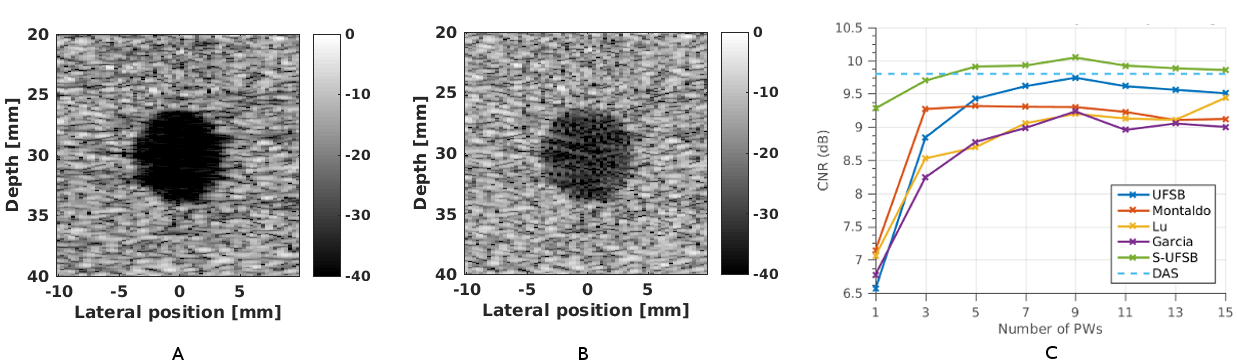
\includegraphics[width=\textwidth]{ResultsIUS3}
\caption{Results obtained by the sparse regularization approach for the 30mm depth Anechoic phantom. (A) and (B) show to the reconstructed images obtained by S-UFSB and UFSB respectively (1 PW). (C) shows the CNR vs the number of PWs for the compounding scheme.}
\label{fig:ResSparse}
\end{figure*}

\subsection{Spatial Resolution}
The spatial resolution is measured using the UlaOp system and a high power probe. The physical phantom involved in this experiment was a 300 $\mu$m nylon wire positioned in a water tank at different depths from the probe. The spatial resolution is evaluated as the First-Width-Half-Max value of the envelope image both in axial and lateral directions \cite{vanWijk_ULT_2002}. The results are reported on Table \ref{tab:LatRes_depth}. 

\begin{table*}[htb]
\caption{Spatial resolution values measured from the UlaOP scanner with high power probe}
\centering
\scalebox{1}{
\begin{tabular}{| M| M| M| M| M| M| M| M| M| M| M| @{}M@{}} 
\hline  
\multirow{2}{*}{Depth} & \multicolumn{2}{M |}{Lu} & \multicolumn{2}{M |}{Garcia} & \multicolumn{2}{M |}{UFSB} & \multicolumn{2}{M |}{Montaldo} & \multicolumn{2}{M |}{S-UFSB} & \\ [1ex]\cline{2-11}
& Axial & Lateral & Axial & Lateral & Axial & Lateral & Axial & Lateral & Axial & Lateral & \\\hline
 25 mm & $0.4$ mm & $0.7$ mm & $0.4$ mm & $0.6$ mm & $0.4$ mm & $0.7$ mm & $0.4$ mm & $0.6$ mm & $0.3$ mm & $0.6$ mm & \\ 
 35 mm & $0.7$ mm & $0.7$ mm & $0.7$ mm & $0.7$ mm & $0.7$ mm & $0.7$ mm & $0.7$ mm & $0.7$ mm & $0.5$ mm & $0.6$ mm & \\
 45 mm & $0.6$ mm & $1$ mm & $0.6$ mm & $1$ mm & $0.6$ mm & $0.9$ mm & $0.6$ mm & $1$ mm & $0.6$ mm & $1$ mm & \\ \hline
\end{tabular}}
\label{tab:LatRes_depth}
\end{table*}
One can observe that the S-UFSB does not exhibit better resolution. The axial resolution is almost the same for all depths and closed to 0.6 mm which is the order of magnitude of the excitation pulse length. The lateral resolution slightly increases with depth but no noticeable difference is observed with S-UFSB. This was expected since no mathematical effort is made to include a relaxation onto the measurement operator as it could be done in deconvolution problems \cite{Morin_ICIP_2013}.

On figure \ref{fig:PSF}, the PSF of the proposed method is displayed for a 25 mm depth wire phantom. It can be seen that the side lobes of the PSF are greatly reduced with the proposed approach compared to classical UFSB. 
\begin{figure}[htb]
\centering    
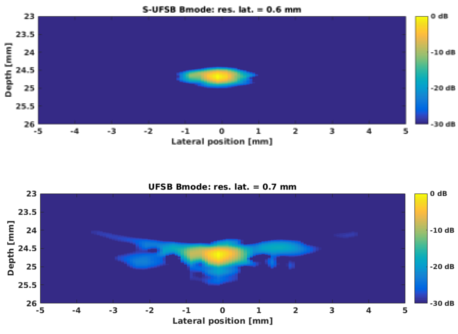
\includegraphics[scale = 0.8]{SpatialRes}
\caption{Point Spread Function obtained with S-UFSB (up) and UFSB (down).}
\label{fig:PSF}
\end{figure}

\section{Conclusion}
\label{sec:Conc}
In this paper, a novel approach for Fourier-based beamforming is proposed. Exploiting sparsity of US images in a Sparsity averaging model, it allows to recover high quality images using $\ell_{1}$-minimization algorithm. This leads to an increase of the CNR of approximately 2dB compared to all the Fourier-based and Space-based techniques for 1 insonifications, while keeping the same spatial resolution. It also enables same contrast as classical DAS method with only 5 PWs. However, the price to pay is a higher computational cost during the reconstruction since solving the $\ell_1$ minimization problem involves an iterative algorithm. 

\section*{Acknowledgements}
This work was supported in part by the UltrasoundToGo RTD project (no. 20NA21 145911), evaluated by the Swiss NSF and funded by Nano-Tera.ch with Swiss Confederation financing. This work was also performed within the framework of the LABEX PRIMES (ANR- 11-LABX-0063) of Universite de Lyon, within the program ”Investissements d’Avenir” (ANR-11-IDEX-0007) operated by the French National Research Agency (ANR).

\bibliographystyle{ieeetr}
\bibliography{IUS2015}

\end{document}


